\subsection{\bt{Data-change scenarios with LLM agents}{大模型智能体的数据变化场景}}
\label{sec:scenarios}
\bi{\emph{Protocol (Q5).} Five metrics (store revenue, store return amount, store return rate, catalog revenue, electronics store revenue) each have two learning questions and three scored questions: a new period, a period difference, and a monthly ranking. \system's built-in analysis optimizer answers the learning questions with explicit business definitions, and judged-successful trajectories pass extraction and admission. A user agent that has never seen the metrics answers the scored questions given only metric names, first on unchanged data and then once per data-change scenario; each scenario starts from the same snapshot and store, applies one update, re-asks the questions whose metric reads an updated table, and is rolled back. Reference answers reflect the update's business effect, so an agent must filter out duplicate rows, status rows, backup copies, or old versions. The eleven scenarios of Figure~\ref{fig:scenarios} are four benign updates (a month of sales appended, late-arriving returns, an in-place correction, an empty new column), five covered breaks (an application-state row per return, restated sales kept as non-current rows, a duplicate load of four months, SCD Type 2 rows in the item dimension, sales whose date keys use another format), the unit change (amounts multiplied by 100 from one month on), which no condition covers, and the backup copy of Section~\ref{sec:repair-eval}.}
{\emph{实验流程（Q5）。}5 个指标（门店营业额、门店退货金额、门店退货率、目录渠道营业额、电子品类门店营业额）各有 2 道学习题和 3 道计分题：新期间、跨期差值和按月排名。\system\ 内置的分析优化器在给出显式业务定义的学习题上作答，判题成功的轨迹经提取与准入后发布。从未接触过这些指标的用户端智能体只拿到指标名，先在未变化的数据上回答计分题，再在每个数据变化场景下各答一次；每个场景从相同的快照和知识库出发，施加一次更新，只重问读到被更新表的指标，结束后回滚。标准答案反映更新的业务效果，因此智能体必须过滤掉重复行、状态行、备份副本或旧版本。图~\ref{fig:scenarios} 的 11 个场景是 4 种正常更新（追加一个月销售、迟到的退货、原地更正、新增空列），5 种条件覆盖的破坏（每笔退货追加申请状态行、旧版本销售保留为非当前行、四个月销售重复加载、商品维度增加缓慢变化维类型 2 的旧版本行、追加日期键为另一种格式的销售），任何条件都不覆盖的单位变化（某月起金额乘以 100），以及第~\ref{sec:repair-eval} 节的备份副本。}

\bi{\emph{Methods and runs.} Besides the strategies of Table~\ref{tab:ladder}, a matched \emph{example-retrieval} baseline in the spirit of AgentSM~\cite{biswal2026agentsm} receives the same learning tasks under the same admission precondition, stores the question, the SQL that produced the answer, and its derivation, and lets the user agent retrieve up to three examples by question similarity, without validity maintenance. Agent and extractor use DeepSeek V4.1 Flash with high reasoning effort, a 20-turn limit, and a 60\,s SQL timeout. Each of the nine methods runs three times, and every run learns its own library. We analyze \ScenCells\ runs with \ScenValidTasks\ scored tasks (\ScenTokensM\,M tokens; \ScenQuotaTasks\ tasks that failed with provider errors are not scored); intervals are 95\% bootstrap intervals over whole runs, and the comparison with example retrieval was specified before the runs.}
{\emph{方法与运行。}除表~\ref{tab:ladder} 的维护方式外，一个仿照 AgentSM~\cite{biswal2026agentsm} 的匹配\emph{示例检索}基线获得同样的学习题、同样的入库前提，保存题面、产生答案的 SQL 与算式，用户端智能体按题面相似度检索最多 3 条，不做有效性维护。智能体与提取器使用 DeepSeek V4.1 Flash，推理强度 high，每题最多 20 轮，SQL 超时 60 秒。9 种方法各运行 3 次，每次各自学习自己的定义库。我们分析 \ScenCells\ 次运行、\ScenValidTasks\ 道计分题（\ScenTokensM\,M token；因服务错误失败的 \ScenQuotaTasks\ 道题不计分）；区间为按运行整体重抽样的 95\% 自助法区间，与示例检索的比较在运行前确定。}

\begin{figure*}[t]
\centering
% Vector drawing generated by tools/figures/build.py; rerun it after changing the figure.
\ifbilingual
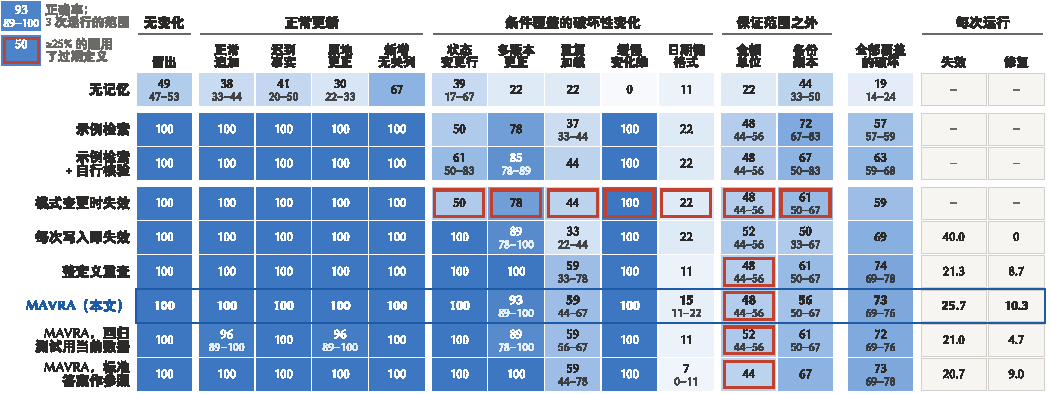
\includegraphics[width=\textwidth]{figures/scenario-changes-zh}
\else
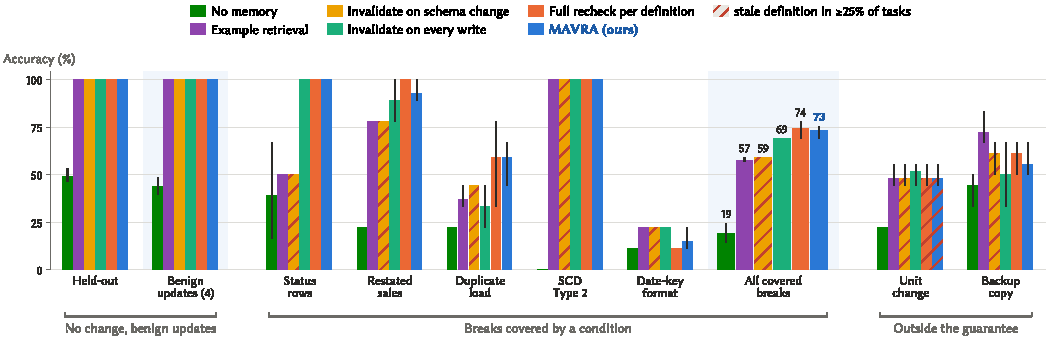
\includegraphics[width=\textwidth]{figures/scenario-changes}
\fi
\caption{\bt{Accuracy of the user agent by data change, DeepSeek V4.1 Flash, for the baselines and \system. Each marker is the accuracy over three independent runs and the line behind it spans the three runs; a red ring marks settings in which at least 25\% of the tasks used a stale definition, i.e., one whose canonical SQL answers that setting's questions incorrectly. Brackets group the changes by the condition they target. Right: invalidations and published repairs per run for the methods that keep definitions, lines spanning the runs; the full recheck and the regression ablation appear only here and in the text. In all, \ScenCells\ runs, \ScenValidTasks\ scored tasks, and \ScenAgentHours\ agent-hours.}{按数据变化划分的用户端智能体正确率，DeepSeek V4.1 Flash，基线与 \system。每个点是 3 次独立运行全部题目上的正确率，点后的细线是 3 次运行的范围；红圈表示该情形下至少 25\% 的题使用了过期定义，即其规范 SQL 在该情形下答错的定义。轴下的括线按变化针对的条件分组。右：维护定义的方法每次运行的失效数与发布的修复数，细线为各次运行的范围；整定义重查与回归测试的消融只出现在这里和正文。共 \ScenCells\ 次运行、\ScenValidTasks\ 道计分题、\ScenAgentHours\ 智能体小时。}}
\label{fig:scenarios}
\Description{Left: a dot plot with the twelve settings on the horizontal axis, grouped by brackets into none, benign, grain, join fan-out, completeness, not covered, and ambiguous fix, and accuracy from 0 to 100 percent on the vertical axis; six methods per setting (no memory, example retrieval, example retrieval with self-verification as diamonds, invalidation on schema change, invalidation on every write, MAVRA), each a marker at the accuracy over runs with a thin line for the range over the three runs. All sharing methods sit at 100 percent on the held-out and benign settings while no memory lies between 30 and 67 percent. Under status-change rows MAVRA and invalidation on every write are at 100 percent, example retrieval and invalidation on schema change at 50, the latter with a red ring, self-verification at 61. Under restatements MAVRA is at 93, every write at 89, example retrieval and schema change at 78 (red ring); under duplicate loads MAVRA at 59, example retrieval at 37, schema change at 44 (red ring), every write at 33. Under SCD Type 2 every sharing method is at 100, schema change ringed. Under the date-key format change all methods lie between 11 and 22 percent, under the unit change between 44 and 52, and under the backup copy example retrieval is highest at 72 with MAVRA at 56. Right: horizontal bars of invalidations (light) and published repairs (solid) per run with the range over runs: invalidation on every write 40 and 0, MAVRA 25.7 and 10.3, full recheck per definition 21.3 and 8.7, MAVRA with the regression test on current data 21.0 and 4.7.}
\end{figure*}


\bi{\emph{Sharing and benign updates.} Without memory, the user agent answers \DsNoShareAll\% of all questions. Every sharing method transfers what was learned: on held-out questions, \system\ and example retrieval both answer \DsCondHoldout\% (\DsNoShareHoldout\% without sharing), and after the benign updates \system\ keeps \DsCondBenign\%; invalidating on every write keeps \DsRevokeBenign\% only by relearning after every write.}
{\emph{共享与正常更新。}没有记忆时，用户端智能体全部题目答对 \DsNoShareAll\%。各共享方法都能迁移学到的内容：留出题上，\system\ 与示例检索都答对 \DsCondHoldout\%（不共享为 \DsNoShareHoldout\%），正常更新之后 \system\ 保持 \DsCondBenign\%；每次写入即失效也保持 \DsRevokeBenign\%，但要靠每次写入后重新学习。}

\bi{\emph{Covered breaking changes.} Here the methods separate. \system\ answers \DsCondModeled\% (\DsCondModeledLo--\DsCondModeledHi) and example retrieval \DsTrajModeled\%, \DsCmpModeledTraj\ points apart (\DsCmpModeledTrajLo--\DsCmpModeledTrajHi). Retrieved examples carry no validity state: under status-change rows they replay SQL that counts some returns twice (\ScenAccTrajStatus\% against \ScenAccCondStatus\%), and under restatements and duplicate loads they reuse SQL written for the old grain (\ScenAccTrajRevision\% and \ScenAccTrajDupload\%, against \ScenAccCondRevision\% and \ScenAccCondDupload\%). Invalidation on schema change serves stale definitions in \DsSchemaStaleModeled\ tasks (\DsSchemaModeled\%); the revalidation methods serve none and are equally accurate: the full recheck answers \DsDefModeled\% and differs from \system\ only in cost (Section~\ref{sec:cost}). Regression as of learning time matters for automation: \system\ publishes \DsCondRepaired\ repairs per run, against \DsCondCurRepaired\ with the regression test on current data, where agents must re-derive the refused filters themselves (\DsCondCurModeled\%). Telling the example-retrieval agent to verify grain, join keys, and date keys, the properties \system\ checks for it, moves it to \DsTrajVerifyModeled\% at \DsTrajVerifyTurns\ instead of \DsTrajTurns\ turns, still \DsCmpModeledCondVerify\ points behind \system\ (\DsCmpModeledCondVerifyLo--\DsCmpModeledCondVerifyHi): an agent told what to check must still find the distinguishing column and filter in every session, whereas a maintained definition carries the check result and the repair.}
{\emph{条件覆盖的破坏性变化。}各方法在这里拉开差距。\system\ 答对 \DsCondModeled\%（\DsCondModeledLo--\DsCondModeledHi），示例检索 \DsTrajModeled\%，相差 \DsCmpModeledTraj\ 个百分点（\DsCmpModeledTrajLo--\DsCmpModeledTrajHi）。检索到的示例没有有效性状态：状态变更行下它重放会把部分退货算两次的 SQL（\ScenAccTrajStatus\% 对 \ScenAccCondStatus\%）；多版本更正与重复加载下它沿用为旧粒度写的 SQL（\ScenAccTrajRevision\% 与 \ScenAccTrajDupload\%，对 \ScenAccCondRevision\% 与 \ScenAccCondDupload\%）。只在模式变更时失效在 \DsSchemaStaleModeled\ 道题中提供了过期定义（\DsSchemaModeled\%）；各重验证方法一道也没有，且同样准确：整定义重查答对 \DsDefModeled\%，与 \system\ 只在代价上不同（第~\ref{sec:cost} 节）。按学习时刻回归决定了自动化程度：\system\ 每次运行发布 \DsCondRepaired\ 个修复，回归测试用当前数据时只有 \DsCondCurRepaired\ 个，被拒绝的过滤要由智能体自己重新推出（\DsCondCurModeled\%）。让示例检索的智能体核对粒度、连接键与日期键——正是 \system\ 替它检查的性质——使其达到 \DsTrajVerifyModeled\%，每题轮数从 \DsTrajTurns\ 增至 \DsTrajVerifyTurns，仍落后 \system\ \DsCmpModeledCondVerify\ 个百分点（\DsCmpModeledCondVerifyLo--\DsCmpModeledCondVerifyHi）：被告知要检查什么的智能体仍要在每次会话中自己找到区分列和过滤，而维护后的定义带着检查结果和修复。}

\bi{\emph{Controls.} Duplicate loads and the date-key format change are detected and the definitions invalidated, since no filter restores the grain; the unit change violates no condition (\ScenAccCondUnit\% for \system, \ScenAccTrajUnit\% for example retrieval). Under the backup copy the uniqueness rule refuses an ambiguous repair and invalidates the returns definitions; for return rate, which has no definition to fall back on, retrieval keeps its edge (\DsTrajMirror\% against \DsCondMirror\%), the price of invalidating rather than guessing.}
{\emph{对照。}重复加载与日期键格式变化被检测到，定义失效，因为没有过滤能恢复粒度；单位变化不违反任何条件（\system\ 为 \ScenAccCondUnit\%，示例检索为 \ScenAccTrajUnit\%）。备份副本下唯一性规则拒绝有歧义的修复，退货定义失效；对没有定义可以回退的退货率，检索保持优势（\DsTrajMirror\% 对 \DsCondMirror\%），这是使定义失效而不是猜测的代价。}

\bi{\emph{Cost and declared use.} Maintenance database time is dominated by repair searches, which \system\ and the full recheck both perform (\ScenMaintCond\ versus \ScenMaintDef\,s per run); invalidating on every write relearns with \ScenRelearnTok\,M LLM tokens per run. Sharing shortens held-out tasks from \ScenHoldTurnsNoShareModelA\ to \ScenHoldTurnsCondModelA\ turns and cuts input tokens by \ScenHoldTokSaveModelA\%. A separate session study times complete tasks on fixed libraries, including first use, updates, and six-request bursts: \SlSessions\ fresh sessions take \SlCondMean\,s on average with \system\ (\SlCondCorrect\ of \SlCondN\ correct) against \SlNoneMean\,s without shared definitions (\SlNoneCorrect\ of \SlNoneN), and \SlDefMean\ and \SlCacheMean\,s with the full recheck and the query cache, so the saving comes from sharing rather than from the maintenance method. Execution-side checks apply only to declared uses: in the three-LLM study, \DuUndeclPct\% of scored answers declared no definition, and \DuDevPct\% of those that declared a correct revision were still wrong because the agent's SQL deviated from it. On an earlier prototype, maintained sharing raised accuracy for all three LLMs we tried (DeepSeek V4.1 Flash \PrevScenAccNoShareModelA\% to \PrevScenAccCondModelA\%, GLM-5.3 \PrevScenAccNoShareModelB\% to \PrevScenAccCondModelB\%, GLM-5.3 Flash \PrevScenAccNoShareModelC\% to \PrevScenAccCondModelC\%).}
{\emph{代价与声明使用。}维护数据库时间以修复搜索为主，\system\ 与整定义重查都要做（每次运行 \ScenMaintCond\ 秒对 \ScenMaintDef\ 秒）；每次写入即失效每次运行用 \ScenRelearnTok\ 百万个大模型 token 重新学习。共享使留出题每题轮数从 \ScenHoldTurnsNoShareModelA\ 降至 \ScenHoldTurnsCondModelA{}，输入 token 减少 \ScenHoldTokSaveModelA\%。另一个会话实验在固定定义库上计时完整任务，覆盖首次使用、数据更新和六请求突发：\SlSessions\ 个全新会话使用 \system\ 时平均 \SlCondMean\ 秒（\SlCondN\ 题答对 \SlCondCorrect\ 题），没有共享定义时 \SlNoneMean\ 秒（\SlNoneN\ 题答对 \SlNoneCorrect\ 题），整定义重查与查询缓存分别为 \SlDefMean\ 秒和 \SlCacheMean\ 秒，因此节省来自共享而不是维护方式。执行端检查只作用于声明了修订的使用：在三模型实验中，\DuUndeclPct\% 的计分答案没有声明任何定义；在声明了正确修订的答案中仍有 \DuDevPct\% 答错，原因是智能体的 SQL 偏离了定义。在较早的原型上，维护后的共享对我们试过的 3 个大模型都提高了正确率（DeepSeek V4.1 Flash 从 \PrevScenAccNoShareModelA\% 到 \PrevScenAccCondModelA\%，GLM-5.3 从 \PrevScenAccNoShareModelB\% 到 \PrevScenAccCondModelB\%，GLM-5.3 Flash 从 \PrevScenAccNoShareModelC\% 到 \PrevScenAccCondModelC\%）。}
